\section{问题描述与覆盖率分析}
\label{sec:problem}

\subsection{固定预算下的记忆构造问题}
\label{sec:formulation}
在决策时刻 $t$，策略 $\pi_\theta$ 接收当前的前置与腕部图像 $o_t=(I^{f}_t,I^{w}_t)$、本体状态 $s_t$、语言指令 $\ell$ 以及记忆 $\mathcal M_t$，输出动作块
\begin{equation}
A_t=(a_t,\dots,a_{t+H-1})=\pi_\theta(o_t,s_t,\ell,\mathcal M_t),\qquad H=20,
\end{equation}
其中前 \V{exec_h} 步被执行后再进行下一次决策。记忆由一个\emph{记忆构造函数}给出：
\begin{equation}
\mathcal M_t=\Phi\big(I_{0:t};\ \mathcal E_t\big)=\big\{(m_i,\ \tau_i,\ \delta_i)\big\}_{i=1}^{B},
\label{eq:selection}
\end{equation}
其中 $m_i$ 是一幅记忆图像（可以是某一历史帧，也可以是由多帧合成的图像），$\tau_i$ 是它的类型，$\delta_i$ 是它距当前时刻的时龄，$\mathcal E_t$ 是截至 $t$ 时刻检测到的事件集合。我们要求 $\Phi$ 满足两条约束：\emph{因果性}，只使用 $t$ 时刻及以前的信息；\emph{预算不变}，与基础模型一样恰好输出 $B$ 幅记忆图像、每幅编码为相同数量的 token。于是不同记忆方法之间的任何行为差异，只能来自记忆的\emph{内容与组织}，而不是\emph{数量}。本文取 $B=\V{budget_B}$，与基础模型一致。均匀记忆是 $\Phi$ 的最简特例：$m_i$ 取等距的历史帧，$\tau_i$ 恒为“上下文”。

\subsection{农业作业中的两类记忆需求}
\label{sec:two_memories}
采摘作业所需记住的信息可分为性质截然不同的两类。

\begin{definition}[场景记忆与事件记忆]
\emph{场景记忆}指在某些观测时刻存在于环境中、此后可能变得不可见的信息，例如被风吹动的叶片遮住之前的成熟果实。\emph{事件记忆}指由机器人自身的交互产生、只在短暂时刻可观测的信息，例如“刚刚摘下一颗果实”。
\end{definition}

两类信息对记忆的要求不同。场景信息集中出现在回合开始或场景切换后的早期帧中（遮挡往往在作业中逐渐发生），只要保留这些\emph{场景锚}帧即可；事件信息则分散在整个回合中，每次采摘只在约 \V{pick_frames} 帧内可见，其数量随作业时长不断增长。第~\ref{sec:audit} 节的审计表明，通用的均匀记忆对前者已经足够（它总是包含第 0 帧），却无法满足后者。这一区分是 HarvestMem 分层设计的出发点，也决定了我们在基准中分别检验两类任务。

\subsection{均匀记忆的事件覆盖率}
\label{sec:coverage}
设一次已完成采摘 $e$ 的关键集合 $S_e$ 为其接触帧和脱离帧前后各 $W$ 帧内的所有帧，$|S_e|\le 2(2W+1)$；若记忆中至少有一帧落在 $S_e$ 内，称该采摘在 $t$ 时刻被\emph{覆盖}。

\begin{proposition}[均匀记忆的覆盖率衰减]
\label{prop:uniform}
设均匀记忆每隔 $\Delta_t=t/(B-1)$ 帧保留一帧，采样网格的相位与采摘时刻无关，且 $\Delta_t$ 大于每个关键窗口的长度，则一次已完成采摘被覆盖的概率为
\begin{equation}
c_U(t)\approx\min\!\Big(1,\ \frac{(B-1)\,|S_e|}{t}\Big).
\label{eq:coverage}
\end{equation}
\end{proposition}
\noindent\emph{说明。}每个关键窗口长度不超过 $\Delta_t$ 时至多落入一帧采样点，落入的概率为窗口长度与 $\Delta_t$ 之比；两个窗口的贡献相加即得式~(\ref{eq:coverage})。

命题~\ref{prop:uniform} 有三个对采摘作业至关重要的推论。第一，\textbf{遗忘随作业时长加剧}：预算固定时覆盖率按 $1/t$ 衰减，最近一次采摘也得不到任何保护。第二，\textbf{记得住的采摘次数存在上限}：$n$ 次采摘中期望被覆盖的次数为 $n\,c_U(t)$，而 $t$ 与 $n$ 近似成正比，因此该数量趋于常数 $(B-1)|S_e|/\bar g$（$\bar g$ 为相邻采摘的平均间隔）；对本文的任务约为 \V{cap_u} 次，与已摘多少颗无关（图~\ref{fig:capacity}）。第三，\textbf{靠扩大预算补救代价高昂}：要维持覆盖率 $c$，需要 $B\ge 1+c\,t/|S_e|$；取 $W=3$（$|S_e|=14$）、$t=600$，完全覆盖约需 44 帧，接近基础预算的 3 倍，注意力开销随之按平方增长。

按事件索引记忆可以消除对 $t$ 的依赖，但最直接的做法，即为最近的采摘预留接触帧和脱离帧（下称\emph{平坦事件关键帧}，记为 \pekm{}，$k$ 为预留帧数上限），每次采摘恒定占用两个位置。为保留场景锚和最基本的时间上下文，16 帧预算最多只能覆盖 \V{cap_flat_max} 次采摘；常用的 $k=8$ 设置只能覆盖最近 4 次。一株番茄的一轮采收往往需要摘下 10 颗以上，一行植株的作业则以数十次计，因此平坦方案的容量远不能满足农业作业的需求。要在预算不变的前提下记住更多采摘，必须\emph{压缩}远期事件，这正是第~\ref{sec:hem} 节分层记忆要解决的问题。

图~\ref{fig:timeline} 用一个真实的验证回合展示了均匀记忆的失效机制（回合编号固定为 0，并非挑选）。均匀记忆的等距网格恰好落在第 2 次和第 4 次采摘上，却从第 1 次和第 3 次采摘的接触帧与脱离帧之间穿过；在最后一次决策时，记忆中只有 4 次采摘中 2 次的证据，篮中果数无法从记忆中恢复。第~\ref{sec:res_memory} 节将在全部验证数据上定量检验命题~\ref{prop:uniform}。

\begin{figure}[t]
\centering
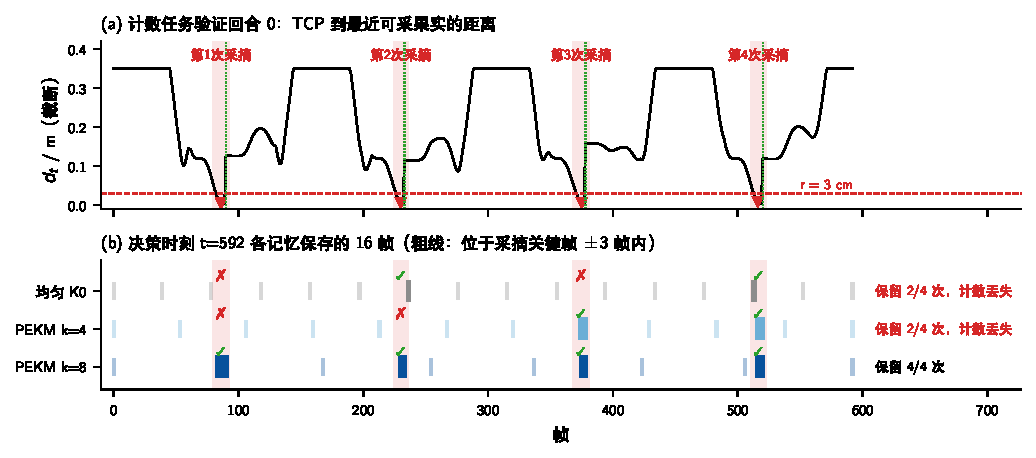
\includegraphics[width=\linewidth]{zh_timeline}
\caption{16 帧记忆实际保存了什么（真实数据，v1 计数任务验证回合 0）。(a) TCP 到最近可采果实的距离 $d_t$，阴影为采摘及其 $\pm 3$ 帧关键窗口，三角为接触关键帧，红色虚线为半径 $r$，绿色点线为果实脱离时刻。(b) 最后一次决策时各记忆保存的帧，粗线表示位于接触或脱离关键帧 $\pm3$ 帧以内，\checkmark/$\times$ 表示该次采摘是否被覆盖。}
\label{fig:timeline}
\end{figure}
